\documentclass[1p]{elsarticle_modified}
%\bibliographystyle{elsarticle-num}

%\usepackage[colorlinks]{hyperref}
%\usepackage{abbrmath_seonhwa} %\Abb, \Ascr, \Acal ,\Abf, \Afrak
\usepackage{amsfonts}
\usepackage{amssymb}
\usepackage{amsmath}
\usepackage{amsthm}
\usepackage{scalefnt}
\usepackage{amsbsy}
\usepackage{kotex}
\usepackage{caption}
\usepackage{subfig}
\usepackage{color}
\usepackage{graphicx}
\usepackage{xcolor} %% white, black, red, green, blue, cyan, magenta, yellow
\usepackage{float}
\usepackage{setspace}
\usepackage{hyperref}

\usepackage{tikz}
\usetikzlibrary{arrows}

\usepackage{multirow}
\usepackage{array} % fixed length table
\usepackage{hhline}

%%%%%%%%%%%%%%%%%%%%%
\makeatletter
\renewcommand*\env@matrix[1][\arraystretch]{%
	\edef\arraystretch{#1}%
	\hskip -\arraycolsep
	\let\@ifnextchar\new@ifnextchar
	\array{*\c@MaxMatrixCols c}}
\makeatother %https://tex.stackexchange.com/questions/14071/how-can-i-increase-the-line-spacing-in-a-matrix
%%%%%%%%%%%%%%%

\usepackage[normalem]{ulem}

\newcommand{\msout}[1]{\ifmmode\text{\sout{\ensuremath{#1}}}\else\sout{#1}\fi}
%SOURCE: \msout is \stkout macro in https://tex.stackexchange.com/questions/20609/strikeout-in-math-mode

\newcommand{\cancel}[1]{
	\ifmmode
	{\color{red}\msout{#1}}
	\else
	{\color{red}\sout{#1}}
	\fi
}

\newcommand{\add}[1]{
	{\color{blue}\uwave{#1}}
}

\newcommand{\replace}[2]{
	\ifmmode
	{\color{red}\msout{#1}}{\color{blue}\uwave{#2}}
	\else
	{\color{red}\sout{#1}}{\color{blue}\uwave{#2}}
	\fi
}

\newcommand{\Sol}{\mathcal{S}} %segment
\newcommand{\D}{D} %diagram
\newcommand{\A}{\mathcal{A}} %arc


%%%%%%%%%%%%%%%%%%%%%%%%%%%%%5 test

\def\sl{\operatorname{\textup{SL}}(2,\Cbb)}
\def\psl{\operatorname{\textup{PSL}}(2,\Cbb)}
\def\quan{\mkern 1mu \triangleright \mkern 1mu}

\theoremstyle{definition}
\newtheorem{thm}{Theorem}[section]
\newtheorem{prop}[thm]{Proposition}
\newtheorem{lem}[thm]{Lemma}
\newtheorem{ques}[thm]{Question}
\newtheorem{cor}[thm]{Corollary}
\newtheorem{defn}[thm]{Definition}
\newtheorem{exam}[thm]{Example}
\newtheorem{rmk}[thm]{Remark}
\newtheorem{alg}[thm]{Algorithm}

\newcommand{\I}{\sqrt{-1}}
\begin{document}

%\begin{frontmatter}
%
%\title{Boundary parabolic representations of knots up to 8 crossings}
%
%%% Group authors per affiliation:
%\author{Yunhi Cho} 
%\address{Department of Mathematics, University of Seoul, Seoul, Korea}
%\ead{yhcho@uos.ac.kr}
%
%
%\author{Seonhwa Kim} %\fnref{s_kim}}
%\address{Center for Geometry and Physics, Institute for Basic Science, Pohang, 37673, Korea}
%\ead{ryeona17@ibs.re.kr}
%
%\author{Hyuk Kim}
%\address{Department of Mathematical Sciences, Seoul National University, Seoul 08826, Korea}
%\ead{hyukkim@snu.ac.kr}
%
%\author{Seokbeom Yoon}
%\address{Department of Mathematical Sciences, Seoul National University, Seoul, 08826,  Korea}
%\ead{sbyoon15@snu.ac.kr}
%
%\begin{abstract}
%We find all boundary parabolic representation of knots up to 8 crossings.
%
%\end{abstract}
%\begin{keyword}
%    \MSC[2010] 57M25 
%\end{keyword}
%
%\end{frontmatter}

%\linenumbers
%\tableofcontents
%
\newcommand\colored[1]{\textcolor{white}{\rule[-0.35ex]{0.8em}{1.4ex}}\kern-0.8em\color{red} #1}%
%\newcommand\colored[1]{\textcolor{white}{ #1}\kern-2.17ex	\textcolor{white}{ #1}\kern-1.81ex	\textcolor{white}{ #1}\kern-2.15ex\color{red}#1	}

{\Large $\underline{12n_{0614}~(K12n_{0614})}$}

\setlength{\tabcolsep}{10pt}
\renewcommand{\arraystretch}{1.6}
\vspace{1cm}\begin{tabular}{m{100pt}>{\centering\arraybackslash}m{274pt}}
\multirow{5}{120pt}{
	\centering
	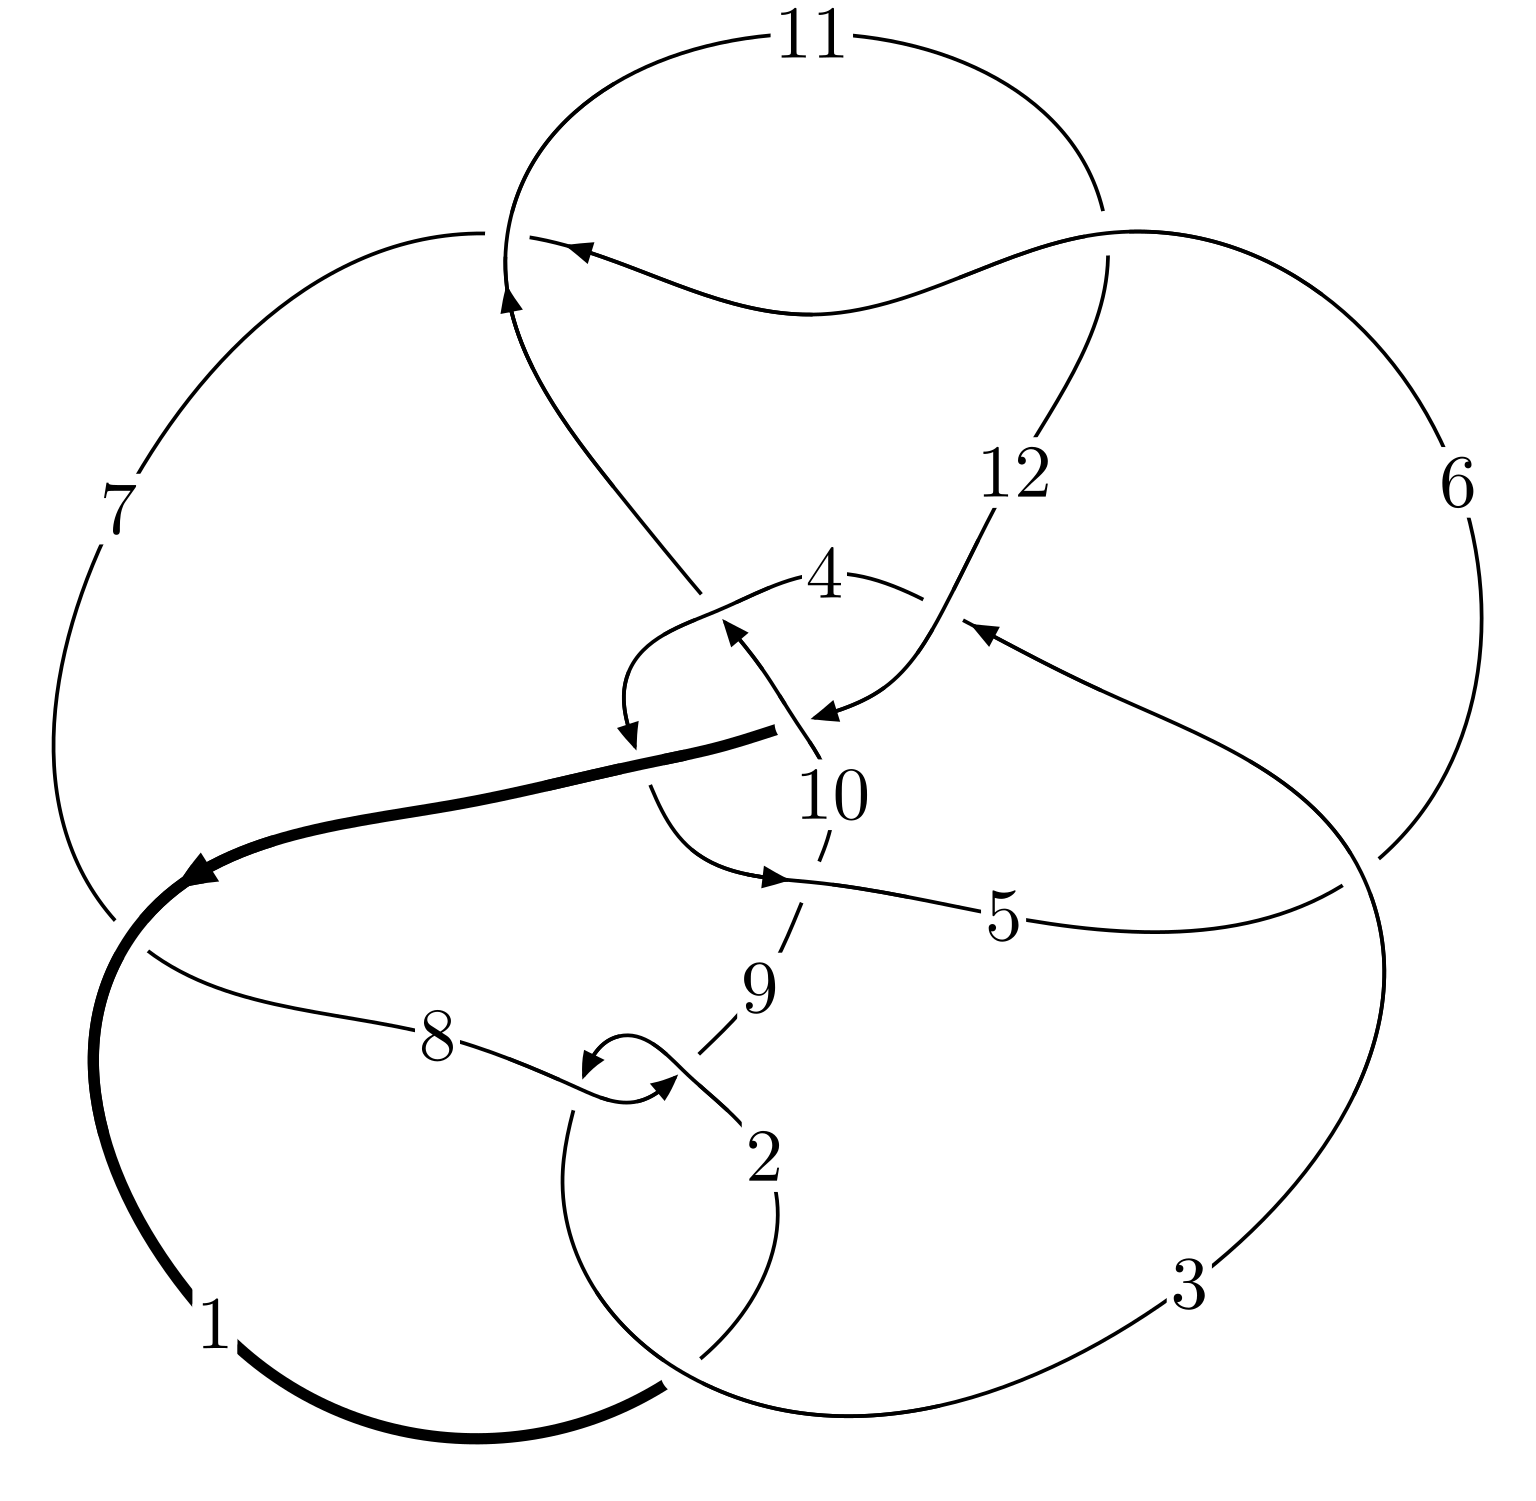
\includegraphics[width=112pt]{../../../GIT/diagram.site/Diagrams/png/2703_12n_0614.png}\\
\ \ \ A knot diagram\footnotemark}&
\allowdisplaybreaks
\textbf{Linearized knot diagam} \\
\cline{2-2}
 &
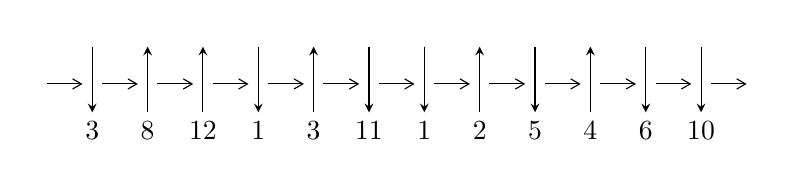
\begin{tikzpicture}[x=20pt, y=17pt]
	% nodes
	\node (C0) at (0, 0) {};
	\node (C1) at (1, 0) {};
	\node (C1U) at (1, +1) {};
	\node (C1D) at (1, -1) {3};

	\node (C2) at (2, 0) {};
	\node (C2U) at (2, +1) {};
	\node (C2D) at (2, -1) {8};

	\node (C3) at (3, 0) {};
	\node (C3U) at (3, +1) {};
	\node (C3D) at (3, -1) {12};

	\node (C4) at (4, 0) {};
	\node (C4U) at (4, +1) {};
	\node (C4D) at (4, -1) {1};

	\node (C5) at (5, 0) {};
	\node (C5U) at (5, +1) {};
	\node (C5D) at (5, -1) {3};

	\node (C6) at (6, 0) {};
	\node (C6U) at (6, +1) {};
	\node (C6D) at (6, -1) {11};

	\node (C7) at (7, 0) {};
	\node (C7U) at (7, +1) {};
	\node (C7D) at (7, -1) {1};

	\node (C8) at (8, 0) {};
	\node (C8U) at (8, +1) {};
	\node (C8D) at (8, -1) {2};

	\node (C9) at (9, 0) {};
	\node (C9U) at (9, +1) {};
	\node (C9D) at (9, -1) {5};

	\node (C10) at (10, 0) {};
	\node (C10U) at (10, +1) {};
	\node (C10D) at (10, -1) {4};

	\node (C11) at (11, 0) {};
	\node (C11U) at (11, +1) {};
	\node (C11D) at (11, -1) {6};

	\node (C12) at (12, 0) {};
	\node (C12U) at (12, +1) {};
	\node (C12D) at (12, -1) {10};
	\node (C13) at (13, 0) {};

	% arrows
	\draw[->,>={angle 60}]
	(C0) edge (C1) (C1) edge (C2) (C2) edge (C3) (C3) edge (C4) (C4) edge (C5) (C5) edge (C6) (C6) edge (C7) (C7) edge (C8) (C8) edge (C9) (C9) edge (C10) (C10) edge (C11) (C11) edge (C12) (C12) edge (C13) ;	\draw[->,>=stealth]
	(C1U) edge (C1D) (C2D) edge (C2U) (C3D) edge (C3U) (C4U) edge (C4D) (C5D) edge (C5U) (C6U) edge (C6D) (C7U) edge (C7D) (C8D) edge (C8U) (C9U) edge (C9D) (C10D) edge (C10U) (C11U) edge (C11D) (C12U) edge (C12D) ;
	\end{tikzpicture} \\
\hhline{~~} \\& 
\textbf{Solving Sequence} \\ \cline{2-2} 
 &
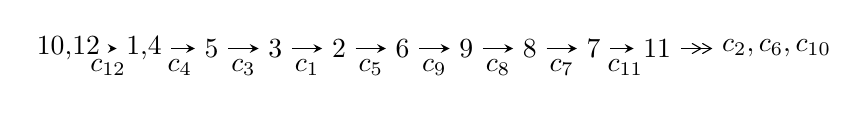
\begin{tikzpicture}[x=23pt, y=7pt]
	% node
	\node (A0) at (-1/8, 0) {10,12};
	\node (A1) at (17/16, 0) {1,4};
	\node (A2) at (17/8, 0) {5};
	\node (A3) at (25/8, 0) {3};
	\node (A4) at (33/8, 0) {2};
	\node (A5) at (41/8, 0) {6};
	\node (A6) at (49/8, 0) {9};
	\node (A7) at (57/8, 0) {8};
	\node (A8) at (65/8, 0) {7};
	\node (A9) at (73/8, 0) {11};
	\node (C1) at (1/2, -1) {$c_{12}$};
	\node (C2) at (13/8, -1) {$c_{4}$};
	\node (C3) at (21/8, -1) {$c_{3}$};
	\node (C4) at (29/8, -1) {$c_{1}$};
	\node (C5) at (37/8, -1) {$c_{5}$};
	\node (C6) at (45/8, -1) {$c_{9}$};
	\node (C7) at (53/8, -1) {$c_{8}$};
	\node (C8) at (61/8, -1) {$c_{7}$};
	\node (C9) at (69/8, -1) {$c_{11}$};
	\node (A10) at (11, 0) {$c_{2},c_{6},c_{10}$};

	% edge
	\draw[->,>=stealth]	
	(A0) edge (A1) (A1) edge (A2) (A2) edge (A3) (A3) edge (A4) (A4) edge (A5) (A5) edge (A6) (A6) edge (A7) (A7) edge (A8) (A8) edge (A9) ;
	\draw[->>,>={angle 60}]	
	(A9) edge (A10);
\end{tikzpicture} \\ 

\end{tabular} \\

\footnotetext{
The image of knot diagram is generated by the software ``\textbf{Draw programme}" developed by Andrew Bartholomew(\url{http://www.layer8.co.uk/maths/draw/index.htm\#Running-draw}), where we modified some parts for our purpose(\url{https://github.com/CATsTAILs/LinksPainter}).
}\phantom \\ \newline 
\centering \textbf{Ideals for irreducible components\footnotemark of $X_{\text{par}}$} 
 
\begin{align*}
I^u_{1}&=\langle 
-2.58062\times10^{138} u^{65}+4.69453\times10^{138} u^{64}+\cdots+1.96428\times10^{138} b-6.10934\times10^{138},\\
\phantom{I^u_{1}}&\phantom{= \langle  }-5.77959\times10^{138} u^{65}+1.53536\times10^{139} u^{64}+\cdots+1.96428\times10^{138} a-8.78790\times10^{138},\;u^{66}-3 u^{65}+\cdots- u+1\rangle \\
I^u_{2}&=\langle 
-2.51011\times10^{19} u^{29}-1.59153\times10^{20} u^{28}+\cdots+4.01614\times10^{18} b+6.48608\times10^{19},\\
\phantom{I^u_{2}}&\phantom{= \langle  }9.77600\times10^{19} u^{29}+6.23565\times10^{20} u^{28}+\cdots+4.01614\times10^{18} a-2.61075\times10^{20},\;u^{30}+6 u^{29}+\cdots-5 u+1\rangle \\
\\
\end{align*}
\raggedright * 2 irreducible components of $\dim_{\mathbb{C}}=0$, with total 96 representations.\\
\footnotetext{All coefficients of polynomials are rational numbers. But the coefficients are sometimes approximated in decimal forms when there is not enough margin.}
\newpage
\renewcommand{\arraystretch}{1}
\centering \section*{I. $I^u_{1}= \langle -2.58\times10^{138} u^{65}+4.69\times10^{138} u^{64}+\cdots+1.96\times10^{138} b-6.11\times10^{138},\;-5.78\times10^{138} u^{65}+1.54\times10^{139} u^{64}+\cdots+1.96\times10^{138} a-8.79\times10^{138},\;u^{66}-3 u^{65}+\cdots- u+1 \rangle$}
\flushleft \textbf{(i) Arc colorings}\\
\begin{tabular}{m{7pt} m{180pt} m{7pt} m{180pt} }
\flushright $a_{10}=$&$\begin{pmatrix}0\\u\end{pmatrix}$ \\
\flushright $a_{12}=$&$\begin{pmatrix}1\\0\end{pmatrix}$ \\
\flushright $a_{1}=$&$\begin{pmatrix}1\\u^2\end{pmatrix}$ \\
\flushright $a_{4}=$&$\begin{pmatrix}2.94235 u^{65}-7.81641 u^{64}+\cdots+25.6075 u+4.47386\\1.31378 u^{65}-2.38995 u^{64}+\cdots-2.35764 u+3.11022\end{pmatrix}$ \\
\flushright $a_{5}=$&$\begin{pmatrix}1.35304 u^{65}-5.33630 u^{64}+\cdots+26.0334 u+0.352996\\1.00899 u^{65}-0.212160 u^{64}+\cdots-3.05615 u+5.39804\end{pmatrix}$ \\
\flushright $a_{3}=$&$\begin{pmatrix}1.62857 u^{65}-5.42646 u^{64}+\cdots+27.9652 u+1.36363\\1.31378 u^{65}-2.38995 u^{64}+\cdots-2.35764 u+3.11022\end{pmatrix}$ \\
\flushright $a_{2}=$&$\begin{pmatrix}2.67431 u^{65}-6.60681 u^{64}+\cdots+7.51766 u+0.766700\\-1.06116 u^{65}+2.61339 u^{64}+\cdots-4.02289 u+2.44879\end{pmatrix}$ \\
\flushright $a_{6}=$&$\begin{pmatrix}2.56600 u^{65}-6.01019 u^{64}+\cdots+22.5310 u+4.35095\\0.291260 u^{65}-1.82499 u^{64}+\cdots-2.83835 u-0.458853\end{pmatrix}$ \\
\flushright $a_{9}=$&$\begin{pmatrix}-1.65301 u^{65}+3.65430 u^{64}+\cdots-1.56313 u+1.16438\\0.868094 u^{65}-1.36078 u^{64}+\cdots+2.50443 u-0.692763\end{pmatrix}$ \\
\flushright $a_{8}=$&$\begin{pmatrix}-2.32081 u^{65}+5.95599 u^{64}+\cdots-22.5004 u+1.37356\\2.29981 u^{65}-4.87483 u^{64}+\cdots+9.45129 u-0.967867\end{pmatrix}$ \\
\flushright $a_{7}=$&$\begin{pmatrix}0.411567 u^{65}-0.846993 u^{64}+\cdots-14.3635 u-0.600756\\1.53761 u^{65}-4.15828 u^{64}+\cdots+8.11307 u-2.36203\end{pmatrix}$ \\
\flushright $a_{11}=$&$\begin{pmatrix}-0.387409 u^{65}-0.881551 u^{64}+\cdots+2.81929 u-2.83069\\-0.986797 u^{65}+2.57596 u^{64}+\cdots+2.56990 u+0.0462032\end{pmatrix}$\\&\end{tabular}
\flushleft \textbf{(ii) Obstruction class $= -1$}\\~\\
\flushleft \textbf{(iii) Cusp Shapes $= 10.6441 u^{65}-22.9856 u^{64}+\cdots+3.38658 u+10.7302$}\\~\\
\newpage\renewcommand{\arraystretch}{1}
\flushleft \textbf{(iv) u-Polynomials at the component}\newline \\
\begin{tabular}{m{50pt}|m{274pt}}
Crossings & \hspace{64pt}u-Polynomials at each crossing \\
\hline $$\begin{aligned}c_{1}\end{aligned}$$&$\begin{aligned}
&u^{66}+15 u^{65}+\cdots-3 u+1
\end{aligned}$\\
\hline $$\begin{aligned}c_{2},c_{8}\end{aligned}$$&$\begin{aligned}
&u^{66}+u^{65}+\cdots+15 u+1
\end{aligned}$\\
\hline $$\begin{aligned}c_{3}\end{aligned}$$&$\begin{aligned}
&u^{66}+3 u^{65}+\cdots+17224 u+1571
\end{aligned}$\\
\hline $$\begin{aligned}c_{4}\end{aligned}$$&$\begin{aligned}
&u^{66}+2 u^{65}+\cdots-19824143 u+13993901
\end{aligned}$\\
\hline $$\begin{aligned}c_{5}\end{aligned}$$&$\begin{aligned}
&u^{66}-8 u^{65}+\cdots+438 u+29
\end{aligned}$\\
\hline $$\begin{aligned}c_{6},c_{11}\end{aligned}$$&$\begin{aligned}
&u^{66}+28 u^{64}+\cdots-13 u+1
\end{aligned}$\\
\hline $$\begin{aligned}c_{7}\end{aligned}$$&$\begin{aligned}
&u^{66}- u^{65}+\cdots+296940149 u+21005497
\end{aligned}$\\
\hline $$\begin{aligned}c_{9}\end{aligned}$$&$\begin{aligned}
&u^{66}-4 u^{65}+\cdots-10934824 u+2425663
\end{aligned}$\\
\hline $$\begin{aligned}c_{10}\end{aligned}$$&$\begin{aligned}
&u^{66}- u^{65}+\cdots+10841 u+4167
\end{aligned}$\\
\hline $$\begin{aligned}c_{12}\end{aligned}$$&$\begin{aligned}
&u^{66}-3 u^{65}+\cdots- u+1
\end{aligned}$\\
\hline
\end{tabular}\\~\\
\newpage\renewcommand{\arraystretch}{1}
\flushleft \textbf{(v) Riley Polynomials at the component}\newline \\
\begin{tabular}{m{50pt}|m{274pt}}
Crossings & \hspace{64pt}Riley Polynomials at each crossing \\
\hline $$\begin{aligned}c_{1}\end{aligned}$$&$\begin{aligned}
&y^{66}+87 y^{65}+\cdots+221 y+1
\end{aligned}$\\
\hline $$\begin{aligned}c_{2},c_{8}\end{aligned}$$&$\begin{aligned}
&y^{66}+15 y^{65}+\cdots-3 y+1
\end{aligned}$\\
\hline $$\begin{aligned}c_{3}\end{aligned}$$&$\begin{aligned}
&y^{66}-25 y^{65}+\cdots-67947428 y+2468041
\end{aligned}$\\
\hline $$\begin{aligned}c_{4}\end{aligned}$$&$\begin{aligned}
&y^{66}+52 y^{65}+\cdots-1605005892392269 y+195829265197801
\end{aligned}$\\
\hline $$\begin{aligned}c_{5}\end{aligned}$$&$\begin{aligned}
&y^{66}-102 y^{65}+\cdots-73060 y+841
\end{aligned}$\\
\hline $$\begin{aligned}c_{6},c_{11}\end{aligned}$$&$\begin{aligned}
&y^{66}+56 y^{65}+\cdots-55 y+1
\end{aligned}$\\
\hline $$\begin{aligned}c_{7}\end{aligned}$$&$\begin{aligned}
&y^{66}+165 y^{65}+\cdots+9982498502631681 y+441230904217009
\end{aligned}$\\
\hline $$\begin{aligned}c_{9}\end{aligned}$$&$\begin{aligned}
&y^{66}+96 y^{65}+\cdots-208158950639894 y+5883840989569
\end{aligned}$\\
\hline $$\begin{aligned}c_{10}\end{aligned}$$&$\begin{aligned}
&y^{66}-21 y^{65}+\cdots+301897937 y+17363889
\end{aligned}$\\
\hline $$\begin{aligned}c_{12}\end{aligned}$$&$\begin{aligned}
&y^{66}+7 y^{65}+\cdots+93 y+1
\end{aligned}$\\
\hline
\end{tabular}\\~\\
\newpage\flushleft \textbf{(vi) Complex Volumes and Cusp Shapes}
$$\begin{array}{c|c|c}  
\text{Solutions to }I^u_{1}& \I (\text{vol} + \sqrt{-1}CS) & \text{Cusp shape}\\
 \hline 
\begin{aligned}
u &= \phantom{-}0.249527 + 0.973850 I \\
a &= -0.269984 + 0.352199 I \\
b &= -1.284520 - 0.093761 I\end{aligned}
 & \phantom{-}3.79747 + 2.06731 I & \phantom{-0.000000 } 0 \\ \hline\begin{aligned}
u &= \phantom{-}0.249527 - 0.973850 I \\
a &= -0.269984 - 0.352199 I \\
b &= -1.284520 + 0.093761 I\end{aligned}
 & \phantom{-}3.79747 - 2.06731 I & \phantom{-0.000000 } 0 \\ \hline\begin{aligned}
u &= \phantom{-}0.615318 + 0.828344 I \\
a &= -0.02105 + 1.59803 I \\
b &= -0.727846 + 0.496461 I\end{aligned}
 & \phantom{-}0.55976 - 4.92526 I & \phantom{-0.000000 } 0 \\ \hline\begin{aligned}
u &= \phantom{-}0.615318 - 0.828344 I \\
a &= -0.02105 - 1.59803 I \\
b &= -0.727846 - 0.496461 I\end{aligned}
 & \phantom{-}0.55976 + 4.92526 I & \phantom{-0.000000 } 0 \\ \hline\begin{aligned}
u &= -0.437096 + 0.815557 I \\
a &= \phantom{-}0.405639 - 1.190780 I \\
b &= \phantom{-}1.26009 - 1.96901 I\end{aligned}
 & \phantom{-}12.42740 + 5.70029 I & \phantom{-}3.74452 - 6.12160 I \\ \hline\begin{aligned}
u &= -0.437096 - 0.815557 I \\
a &= \phantom{-}0.405639 + 1.190780 I \\
b &= \phantom{-}1.26009 + 1.96901 I\end{aligned}
 & \phantom{-}12.42740 - 5.70029 I & \phantom{-}3.74452 + 6.12160 I \\ \hline\begin{aligned}
u &= \phantom{-}0.033859 + 0.905828 I \\
a &= \phantom{-}0.686387 + 0.796402 I \\
b &= -0.999476 - 0.290107 I\end{aligned}
 & \phantom{-}3.53265 + 0.97150 I & \phantom{-}4.91841 + 0. I\phantom{ +0.000000I} \\ \hline\begin{aligned}
u &= \phantom{-}0.033859 - 0.905828 I \\
a &= \phantom{-}0.686387 - 0.796402 I \\
b &= -0.999476 + 0.290107 I\end{aligned}
 & \phantom{-}3.53265 - 0.97150 I & \phantom{-}4.91841 + 0. I\phantom{ +0.000000I} \\ \hline\begin{aligned}
u &= -0.682349 + 0.882535 I \\
a &= \phantom{-}0.466401 - 1.133650 I \\
b &= -0.374389 - 1.078440 I\end{aligned}
 & -0.80690 + 2.71270 I & \phantom{-0.000000 } 0 \\ \hline\begin{aligned}
u &= -0.682349 - 0.882535 I \\
a &= \phantom{-}0.466401 + 1.133650 I \\
b &= -0.374389 + 1.078440 I\end{aligned}
 & -0.80690 - 2.71270 I & \phantom{-0.000000 } 0\\
 \hline 
 \end{array}$$\newpage$$\begin{array}{c|c|c}  
\text{Solutions to }I^u_{1}& \I (\text{vol} + \sqrt{-1}CS) & \text{Cusp shape}\\
 \hline 
\begin{aligned}
u &= -0.289401 + 0.832892 I \\
a &= -0.352656 + 1.319950 I \\
b &= -1.34067 + 1.94518 I\end{aligned}
 & \phantom{-}13.15070 - 1.94186 I & \phantom{-}5.70542 - 1.07468 I \\ \hline\begin{aligned}
u &= -0.289401 - 0.832892 I \\
a &= -0.352656 - 1.319950 I \\
b &= -1.34067 - 1.94518 I\end{aligned}
 & \phantom{-}13.15070 + 1.94186 I & \phantom{-}5.70542 + 1.07468 I \\ \hline\begin{aligned}
u &= \phantom{-}0.359145 + 0.783685 I \\
a &= \phantom{-}1.054300 - 0.565207 I \\
b &= -0.734467 - 0.404994 I\end{aligned}
 & \phantom{-}7.06668 + 1.57189 I & \phantom{-}4.29931 - 7.86449 I \\ \hline\begin{aligned}
u &= \phantom{-}0.359145 - 0.783685 I \\
a &= \phantom{-}1.054300 + 0.565207 I \\
b &= -0.734467 + 0.404994 I\end{aligned}
 & \phantom{-}7.06668 - 1.57189 I & \phantom{-}4.29931 + 7.86449 I \\ \hline\begin{aligned}
u &= \phantom{-}0.682707 + 0.513106 I \\
a &= \phantom{-}0.24428 - 2.03609 I \\
b &= \phantom{-}1.067660 - 0.541710 I\end{aligned}
 & \phantom{-}1.63963 - 5.80606 I & -5.45360 + 9.71206 I \\ \hline\begin{aligned}
u &= \phantom{-}0.682707 - 0.513106 I \\
a &= \phantom{-}0.24428 + 2.03609 I \\
b &= \phantom{-}1.067660 + 0.541710 I\end{aligned}
 & \phantom{-}1.63963 + 5.80606 I & -5.45360 - 9.71206 I \\ \hline\begin{aligned}
u &= \phantom{-}0.342573 + 0.774825 I \\
a &= -0.00166 + 1.68586 I \\
b &= -0.98226 + 1.11174 I\end{aligned}
 & \phantom{-}3.76909 - 6.48056 I & \phantom{-}5.17385 + 9.06963 I \\ \hline\begin{aligned}
u &= \phantom{-}0.342573 - 0.774825 I \\
a &= -0.00166 - 1.68586 I \\
b &= -0.98226 - 1.11174 I\end{aligned}
 & \phantom{-}3.76909 + 6.48056 I & \phantom{-}5.17385 - 9.06963 I \\ \hline\begin{aligned}
u &= \phantom{-}0.409070 + 0.741183 I \\
a &= -0.977149 + 0.697862 I \\
b &= \phantom{-}0.686979 + 0.481839 I\end{aligned}
 & \phantom{-}6.87593 - 4.70790 I & \phantom{-}1.11470 - 3.72537 I \\ \hline\begin{aligned}
u &= \phantom{-}0.409070 - 0.741183 I \\
a &= -0.977149 - 0.697862 I \\
b &= \phantom{-}0.686979 - 0.481839 I\end{aligned}
 & \phantom{-}6.87593 + 4.70790 I & \phantom{-}1.11470 + 3.72537 I\\
 \hline 
 \end{array}$$\newpage$$\begin{array}{c|c|c}  
\text{Solutions to }I^u_{1}& \I (\text{vol} + \sqrt{-1}CS) & \text{Cusp shape}\\
 \hline 
\begin{aligned}
u &= \phantom{-}0.601095 + 0.581351 I \\
a &= \phantom{-}0.556911 - 0.409109 I \\
b &= \phantom{-}1.025200 - 0.590189 I\end{aligned}
 & \phantom{-}0.136895 + 0.733623 I & -2.74494 + 0. I\phantom{ +0.000000I} \\ \hline\begin{aligned}
u &= \phantom{-}0.601095 - 0.581351 I \\
a &= \phantom{-}0.556911 + 0.409109 I \\
b &= \phantom{-}1.025200 + 0.590189 I\end{aligned}
 & \phantom{-}0.136895 - 0.733623 I & -2.74494 + 0. I\phantom{ +0.000000I} \\ \hline\begin{aligned}
u &= -0.428271 + 0.713032 I \\
a &= \phantom{-}3.10687 - 0.23646 I \\
b &= -0.770827 - 0.716616 I\end{aligned}
 & \phantom{-}12.07670 - 2.21337 I & \phantom{-}4.41985 - 2.89857 I \\ \hline\begin{aligned}
u &= -0.428271 - 0.713032 I \\
a &= \phantom{-}3.10687 + 0.23646 I \\
b &= -0.770827 + 0.716616 I\end{aligned}
 & \phantom{-}12.07670 + 2.21337 I & \phantom{-}4.41985 + 2.89857 I \\ \hline\begin{aligned}
u &= -0.666391 + 0.960759 I \\
a &= \phantom{-}0.586302 - 0.825625 I \\
b &= -0.342142 - 0.858442 I\end{aligned}
 & -0.64111 + 2.45300 I & \phantom{-0.000000 } 0 \\ \hline\begin{aligned}
u &= -0.666391 - 0.960759 I \\
a &= \phantom{-}0.586302 + 0.825625 I \\
b &= -0.342142 + 0.858442 I\end{aligned}
 & -0.64111 - 2.45300 I & \phantom{-0.000000 } 0 \\ \hline\begin{aligned}
u &= -1.178240 + 0.061260 I \\
a &= \phantom{-}0.663485 + 0.224665 I \\
b &= \phantom{-}0.362141 + 0.169931 I\end{aligned}
 & -2.39687 - 0.04300 I & \phantom{-0.000000 } 0 \\ \hline\begin{aligned}
u &= -1.178240 - 0.061260 I \\
a &= \phantom{-}0.663485 - 0.224665 I \\
b &= \phantom{-}0.362141 - 0.169931 I\end{aligned}
 & -2.39687 + 0.04300 I & \phantom{-0.000000 } 0 \\ \hline\begin{aligned}
u &= -0.978455 + 0.724029 I \\
a &= -0.184249 + 0.739258 I \\
b &= \phantom{-}0.158181 + 1.022200 I\end{aligned}
 & -3.11037 + 0.52815 I & \phantom{-0.000000 } 0 \\ \hline\begin{aligned}
u &= -0.978455 - 0.724029 I \\
a &= -0.184249 - 0.739258 I \\
b &= \phantom{-}0.158181 - 1.022200 I\end{aligned}
 & -3.11037 - 0.52815 I & \phantom{-0.000000 } 0\\
 \hline 
 \end{array}$$\newpage$$\begin{array}{c|c|c}  
\text{Solutions to }I^u_{1}& \I (\text{vol} + \sqrt{-1}CS) & \text{Cusp shape}\\
 \hline 
\begin{aligned}
u &= -0.248792 + 0.713501 I \\
a &= \phantom{-}0.350874 - 1.113190 I \\
b &= -0.795609 - 0.732164 I\end{aligned}
 & \phantom{-}1.05108 + 1.79441 I & \phantom{-}1.95797 - 4.33085 I \\ \hline\begin{aligned}
u &= -0.248792 - 0.713501 I \\
a &= \phantom{-}0.350874 + 1.113190 I \\
b &= -0.795609 + 0.732164 I\end{aligned}
 & \phantom{-}1.05108 - 1.79441 I & \phantom{-}1.95797 + 4.33085 I \\ \hline\begin{aligned}
u &= -0.362005 + 0.647934 I \\
a &= -3.73012 - 0.37278 I \\
b &= \phantom{-}0.704011 + 0.655660 I\end{aligned}
 & \phantom{-}12.40550 + 4.61805 I & \phantom{-}6.00525 - 8.48089 I \\ \hline\begin{aligned}
u &= -0.362005 - 0.647934 I \\
a &= -3.73012 + 0.37278 I \\
b &= \phantom{-}0.704011 - 0.655660 I\end{aligned}
 & \phantom{-}12.40550 - 4.61805 I & \phantom{-}6.00525 + 8.48089 I \\ \hline\begin{aligned}
u &= \phantom{-}0.766631 + 1.026940 I \\
a &= -0.522622 + 0.702186 I \\
b &= -1.51898 + 0.65915 I\end{aligned}
 & \phantom{-}6.16026 - 1.87831 I & \phantom{-0.000000 } 0 \\ \hline\begin{aligned}
u &= \phantom{-}0.766631 - 1.026940 I \\
a &= -0.522622 - 0.702186 I \\
b &= -1.51898 - 0.65915 I\end{aligned}
 & \phantom{-}6.16026 + 1.87831 I & \phantom{-0.000000 } 0 \\ \hline\begin{aligned}
u &= \phantom{-}0.983808 + 0.839486 I \\
a &= \phantom{-}0.647660 - 1.216280 I \\
b &= \phantom{-}1.115270 - 0.152332 I\end{aligned}
 & \phantom{-}5.26486 - 4.65376 I & \phantom{-0.000000 } 0 \\ \hline\begin{aligned}
u &= \phantom{-}0.983808 - 0.839486 I \\
a &= \phantom{-}0.647660 + 1.216280 I \\
b &= \phantom{-}1.115270 + 0.152332 I\end{aligned}
 & \phantom{-}5.26486 + 4.65376 I & \phantom{-0.000000 } 0 \\ \hline\begin{aligned}
u &= \phantom{-}0.053565 + 0.677699 I \\
a &= \phantom{-}0.06723 - 2.16764 I \\
b &= \phantom{-}0.732638 + 0.191707 I\end{aligned}
 & \phantom{-}3.59207 + 4.61001 I & \phantom{-}4.03017 - 6.08936 I \\ \hline\begin{aligned}
u &= \phantom{-}0.053565 - 0.677699 I \\
a &= \phantom{-}0.06723 + 2.16764 I \\
b &= \phantom{-}0.732638 - 0.191707 I\end{aligned}
 & \phantom{-}3.59207 - 4.61001 I & \phantom{-}4.03017 + 6.08936 I\\
 \hline 
 \end{array}$$\newpage$$\begin{array}{c|c|c}  
\text{Solutions to }I^u_{1}& \I (\text{vol} + \sqrt{-1}CS) & \text{Cusp shape}\\
 \hline 
\begin{aligned}
u &= -0.887350 + 1.047850 I \\
a &= -0.389145 + 0.768196 I \\
b &= \phantom{-}0.633717 + 0.991445 I\end{aligned}
 & -2.15650 + 6.27128 I & \phantom{-0.000000 } 0 \\ \hline\begin{aligned}
u &= -0.887350 - 1.047850 I \\
a &= -0.389145 - 0.768196 I \\
b &= \phantom{-}0.633717 - 0.991445 I\end{aligned}
 & -2.15650 - 6.27128 I & \phantom{-0.000000 } 0 \\ \hline\begin{aligned}
u &= \phantom{-}0.935204 + 1.043390 I \\
a &= \phantom{-}0.322460 - 0.784777 I \\
b &= \phantom{-}1.47663 - 0.84266 I\end{aligned}
 & \phantom{-}3.09240 - 7.98201 I & \phantom{-0.000000 } 0 \\ \hline\begin{aligned}
u &= \phantom{-}0.935204 - 1.043390 I \\
a &= \phantom{-}0.322460 + 0.784777 I \\
b &= \phantom{-}1.47663 + 0.84266 I\end{aligned}
 & \phantom{-}3.09240 + 7.98201 I & \phantom{-0.000000 } 0 \\ \hline\begin{aligned}
u &= \phantom{-}0.189006 + 0.539851 I \\
a &= -0.14714 - 1.49703 I \\
b &= \phantom{-}1.65589 - 1.01498 I\end{aligned}
 & \phantom{-}1.81042 - 2.05249 I & \phantom{-}3.67407 + 5.51602 I \\ \hline\begin{aligned}
u &= \phantom{-}0.189006 - 0.539851 I \\
a &= -0.14714 + 1.49703 I \\
b &= \phantom{-}1.65589 + 1.01498 I\end{aligned}
 & \phantom{-}1.81042 + 2.05249 I & \phantom{-}3.67407 - 5.51602 I \\ \hline\begin{aligned}
u &= \phantom{-}0.98278 + 1.07695 I \\
a &= -0.374561 + 0.803029 I \\
b &= -0.920434 - 0.084883 I\end{aligned}
 & \phantom{-}2.95941 + 0.54302 I & \phantom{-0.000000 } 0 \\ \hline\begin{aligned}
u &= \phantom{-}0.98278 - 1.07695 I \\
a &= -0.374561 - 0.803029 I \\
b &= -0.920434 + 0.084883 I\end{aligned}
 & \phantom{-}2.95941 - 0.54302 I & \phantom{-0.000000 } 0 \\ \hline\begin{aligned}
u &= \phantom{-}0.96734 + 1.18586 I \\
a &= -0.189609 + 1.218970 I \\
b &= -1.52025 + 1.03660 I\end{aligned}
 & \phantom{-}15.3119 - 8.5854 I & \phantom{-0.000000 } 0 \\ \hline\begin{aligned}
u &= \phantom{-}0.96734 - 1.18586 I \\
a &= -0.189609 - 1.218970 I \\
b &= -1.52025 - 1.03660 I\end{aligned}
 & \phantom{-}15.3119 + 8.5854 I & \phantom{-0.000000 } 0\\
 \hline 
 \end{array}$$\newpage$$\begin{array}{c|c|c}  
\text{Solutions to }I^u_{1}& \I (\text{vol} + \sqrt{-1}CS) & \text{Cusp shape}\\
 \hline 
\begin{aligned}
u &= \phantom{-}0.97648 + 1.18488 I \\
a &= \phantom{-}0.075593 - 1.252430 I \\
b &= \phantom{-}1.46536 - 1.04892 I\end{aligned}
 & \phantom{-}14.4678 - 15.9965 I & \phantom{-0.000000 } 0 \\ \hline\begin{aligned}
u &= \phantom{-}0.97648 - 1.18488 I \\
a &= \phantom{-}0.075593 + 1.252430 I \\
b &= \phantom{-}1.46536 + 1.04892 I\end{aligned}
 & \phantom{-}14.4678 + 15.9965 I & \phantom{-0.000000 } 0 \\ \hline\begin{aligned}
u &= \phantom{-}1.28242 + 1.00513 I \\
a &= \phantom{-}0.884168 - 0.187959 I \\
b &= \phantom{-}1.226060 + 0.549068 I\end{aligned}
 & \phantom{-}14.3264 + 0.4250 I & \phantom{-0.000000 } 0 \\ \hline\begin{aligned}
u &= \phantom{-}1.28242 - 1.00513 I \\
a &= \phantom{-}0.884168 + 0.187959 I \\
b &= \phantom{-}1.226060 - 0.549068 I\end{aligned}
 & \phantom{-}14.3264 - 0.4250 I & \phantom{-0.000000 } 0 \\ \hline\begin{aligned}
u &= \phantom{-}1.30509 + 0.99681 I \\
a &= -0.812511 + 0.031797 I \\
b &= -1.167660 - 0.660772 I\end{aligned}
 & \phantom{-}13.4708 + 7.8026 I & \phantom{-0.000000 } 0 \\ \hline\begin{aligned}
u &= \phantom{-}1.30509 - 0.99681 I \\
a &= -0.812511 - 0.031797 I \\
b &= -1.167660 + 0.660772 I\end{aligned}
 & \phantom{-}13.4708 - 7.8026 I & \phantom{-0.000000 } 0 \\ \hline\begin{aligned}
u &= -1.13183 + 1.26806 I \\
a &= \phantom{-}0.337985 + 0.720296 I \\
b &= \phantom{-}1.196830 + 0.393471 I\end{aligned}
 & \phantom{-}9.15397 + 8.21782 I & \phantom{-0.000000 } 0 \\ \hline\begin{aligned}
u &= -1.13183 - 1.26806 I \\
a &= \phantom{-}0.337985 - 0.720296 I \\
b &= \phantom{-}1.196830 - 0.393471 I\end{aligned}
 & \phantom{-}9.15397 - 8.21782 I & \phantom{-0.000000 } 0 \\ \hline\begin{aligned}
u &= \phantom{-}0.045507 + 0.282776 I \\
a &= -2.19269 + 1.53645 I \\
b &= \phantom{-}0.730632 + 0.344719 I\end{aligned}
 & -0.20859 - 1.52213 I & -3.23626 + 4.72897 I \\ \hline\begin{aligned}
u &= \phantom{-}0.045507 - 0.282776 I \\
a &= -2.19269 - 1.53645 I \\
b &= \phantom{-}0.730632 - 0.344719 I\end{aligned}
 & -0.20859 + 1.52213 I & -3.23626 - 4.72897 I\\
 \hline 
 \end{array}$$\newpage$$\begin{array}{c|c|c}  
\text{Solutions to }I^u_{1}& \I (\text{vol} + \sqrt{-1}CS) & \text{Cusp shape}\\
 \hline 
\begin{aligned}
u &= -1.16315 + 1.29787 I \\
a &= -0.388674 - 0.556758 I \\
b &= -1.166830 - 0.246261 I\end{aligned}
 & \phantom{-}9.09525 + 0.92745 I & \phantom{-0.000000 } 0 \\ \hline\begin{aligned}
u &= -1.16315 - 1.29787 I \\
a &= -0.388674 + 0.556758 I \\
b &= -1.166830 + 0.246261 I\end{aligned}
 & \phantom{-}9.09525 - 0.92745 I & \phantom{-0.000000 } 0 \\ \hline\begin{aligned}
u &= -0.064829 + 0.176117 I \\
a &= \phantom{-}3.07467 - 0.79403 I \\
b &= \phantom{-}0.307561 - 0.497960 I\end{aligned}
 & -0.217612 + 1.382700 I & -2.39310 - 4.83328 I \\ \hline\begin{aligned}
u &= -0.064829 - 0.176117 I \\
a &= \phantom{-}3.07467 + 0.79403 I \\
b &= \phantom{-}0.307561 + 0.497960 I\end{aligned}
 & -0.217612 - 1.382700 I & -2.39310 + 4.83328 I \\ \hline\begin{aligned}
u &= -1.76296 + 0.61380 I \\
a &= \phantom{-}0.0226134 - 0.1199730 I \\
b &= \phantom{-}0.341515 - 0.207501 I\end{aligned}
 & -4.80865 + 3.88403 I & \phantom{-0.000000 } 0 \\ \hline\begin{aligned}
u &= -1.76296 - 0.61380 I \\
a &= \phantom{-}0.0226134 + 0.1199730 I \\
b &= \phantom{-}0.341515 + 0.207501 I\end{aligned}
 & -4.80865 - 3.88403 I & \phantom{-0.000000 } 0\\
 \hline 
 \end{array}$$\newpage\newpage\renewcommand{\arraystretch}{1}
\centering \section*{II. $I^u_{2}= \langle -2.51\times10^{19} u^{29}-1.59\times10^{20} u^{28}+\cdots+4.02\times10^{18} b+6.49\times10^{19},\;9.78\times10^{19} u^{29}+6.24\times10^{20} u^{28}+\cdots+4.02\times10^{18} a-2.61\times10^{20},\;u^{30}+6 u^{29}+\cdots-5 u+1 \rangle$}
\flushleft \textbf{(i) Arc colorings}\\
\begin{tabular}{m{7pt} m{180pt} m{7pt} m{180pt} }
\flushright $a_{10}=$&$\begin{pmatrix}0\\u\end{pmatrix}$ \\
\flushright $a_{12}=$&$\begin{pmatrix}1\\0\end{pmatrix}$ \\
\flushright $a_{1}=$&$\begin{pmatrix}1\\u^2\end{pmatrix}$ \\
\flushright $a_{4}=$&$\begin{pmatrix}-24.3418 u^{29}-155.265 u^{28}+\cdots-150.976 u+65.0064\\6.25007 u^{29}+39.6284 u^{28}+\cdots+37.3973 u-16.1500\end{pmatrix}$ \\
\flushright $a_{5}=$&$\begin{pmatrix}-33.8102 u^{29}-215.601 u^{28}+\cdots-210.102 u+90.3706\\4.95851 u^{29}+31.7341 u^{28}+\cdots+29.2380 u-12.6245\end{pmatrix}$ \\
\flushright $a_{3}=$&$\begin{pmatrix}-30.5919 u^{29}-194.893 u^{28}+\cdots-188.373 u+81.1565\\6.25007 u^{29}+39.6284 u^{28}+\cdots+37.3973 u-16.1500\end{pmatrix}$ \\
\flushright $a_{2}=$&$\begin{pmatrix}-12.1917 u^{29}-76.9619 u^{28}+\cdots-72.9374 u+39.5688\\-0.602753 u^{29}-4.04941 u^{28}+\cdots-4.64126 u+0.893751\end{pmatrix}$ \\
\flushright $a_{6}=$&$\begin{pmatrix}30.2018 u^{29}+191.789 u^{28}+\cdots+184.852 u-79.1727\\-8.03538 u^{29}-51.0463 u^{28}+\cdots-51.8658 u+22.2080\end{pmatrix}$ \\
\flushright $a_{9}=$&$\begin{pmatrix}28.9293 u^{29}+182.939 u^{28}+\cdots+176.262 u-85.9815\\-0.978784 u^{29}-5.60749 u^{28}+\cdots-5.70367 u+3.91752\end{pmatrix}$ \\
\flushright $a_{8}=$&$\begin{pmatrix}-44.5210 u^{29}-283.726 u^{28}+\cdots-280.369 u+118.761\\8.60468 u^{29}+54.5709 u^{28}+\cdots+55.9046 u-23.6544\end{pmatrix}$ \\
\flushright $a_{7}=$&$\begin{pmatrix}-29.1421 u^{29}-186.256 u^{28}+\cdots-185.982 u+78.5055\\10.7566 u^{29}+68.7177 u^{28}+\cdots+66.5121 u-28.8516\end{pmatrix}$ \\
\flushright $a_{11}=$&$\begin{pmatrix}20.6148 u^{29}+130.865 u^{28}+\cdots+127.785 u-60.3047\\-1.36890 u^{29}-8.61147 u^{28}+\cdots-7.61980 u+5.21974\end{pmatrix}$\\&\end{tabular}
\flushleft \textbf{(ii) Obstruction class $= 1$}\\~\\
\flushleft \textbf{(iii) Cusp Shapes $= \frac{39236244732154106120}{4016136176896476131} u^{29}+\frac{247548470797569329746}{4016136176896476131} u^{28}+\cdots+\frac{198693521190973939460}{4016136176896476131} u-\frac{83331556397087838785}{4016136176896476131}$}\\~\\
\newpage\renewcommand{\arraystretch}{1}
\flushleft \textbf{(iv) u-Polynomials at the component}\newline \\
\begin{tabular}{m{50pt}|m{274pt}}
Crossings & \hspace{64pt}u-Polynomials at each crossing \\
\hline $$\begin{aligned}c_{1}\end{aligned}$$&$\begin{aligned}
&u^{30}-14 u^{29}+\cdots-11 u+1
\end{aligned}$\\
\hline $$\begin{aligned}c_{2}\end{aligned}$$&$\begin{aligned}
&u^{30}+7 u^{28}+\cdots+u+1
\end{aligned}$\\
\hline $$\begin{aligned}c_{3}\end{aligned}$$&$\begin{aligned}
&u^{30}+2 u^{29}+\cdots-2 u+1
\end{aligned}$\\
\hline $$\begin{aligned}c_{4}\end{aligned}$$&$\begin{aligned}
&u^{30}+5 u^{29}+\cdots-3 u+1
\end{aligned}$\\
\hline $$\begin{aligned}c_{5}\end{aligned}$$&$\begin{aligned}
&u^{30}-19 u^{29}+\cdots-1154 u+131
\end{aligned}$\\
\hline $$\begin{aligned}c_{6}\end{aligned}$$&$\begin{aligned}
&u^{30}- u^{29}+\cdots- u+1
\end{aligned}$\\
\hline $$\begin{aligned}c_{7}\end{aligned}$$&$\begin{aligned}
&u^{30}+14 u^{28}+\cdots-11 u+1
\end{aligned}$\\
\hline $$\begin{aligned}c_{8}\end{aligned}$$&$\begin{aligned}
&u^{30}+7 u^{28}+\cdots- u+1
\end{aligned}$\\
\hline $$\begin{aligned}c_{9}\end{aligned}$$&$\begin{aligned}
&u^{30}+u^{29}+\cdots-8 u^2+1
\end{aligned}$\\
\hline $$\begin{aligned}c_{10}\end{aligned}$$&$\begin{aligned}
&u^{30}+3 u^{28}+\cdots- u+1
\end{aligned}$\\
\hline $$\begin{aligned}c_{11}\end{aligned}$$&$\begin{aligned}
&u^{30}+u^{29}+\cdots+u+1
\end{aligned}$\\
\hline $$\begin{aligned}c_{12}\end{aligned}$$&$\begin{aligned}
&u^{30}+6 u^{29}+\cdots-5 u+1
\end{aligned}$\\
\hline
\end{tabular}\\~\\
\newpage\renewcommand{\arraystretch}{1}
\flushleft \textbf{(v) Riley Polynomials at the component}\newline \\
\begin{tabular}{m{50pt}|m{274pt}}
Crossings & \hspace{64pt}Riley Polynomials at each crossing \\
\hline $$\begin{aligned}c_{1}\end{aligned}$$&$\begin{aligned}
&y^{30}+18 y^{29}+\cdots+27 y+1
\end{aligned}$\\
\hline $$\begin{aligned}c_{2},c_{8}\end{aligned}$$&$\begin{aligned}
&y^{30}+14 y^{29}+\cdots+11 y+1
\end{aligned}$\\
\hline $$\begin{aligned}c_{3}\end{aligned}$$&$\begin{aligned}
&y^{30}-2 y^{29}+\cdots-22 y+1
\end{aligned}$\\
\hline $$\begin{aligned}c_{4}\end{aligned}$$&$\begin{aligned}
&y^{30}+3 y^{29}+\cdots-11 y+1
\end{aligned}$\\
\hline $$\begin{aligned}c_{5}\end{aligned}$$&$\begin{aligned}
&y^{30}-31 y^{29}+\cdots-199614 y+17161
\end{aligned}$\\
\hline $$\begin{aligned}c_{6},c_{11}\end{aligned}$$&$\begin{aligned}
&y^{30}+15 y^{29}+\cdots+23 y+1
\end{aligned}$\\
\hline $$\begin{aligned}c_{7}\end{aligned}$$&$\begin{aligned}
&y^{30}+28 y^{29}+\cdots-13 y+1
\end{aligned}$\\
\hline $$\begin{aligned}c_{9}\end{aligned}$$&$\begin{aligned}
&y^{30}+7 y^{29}+\cdots-16 y+1
\end{aligned}$\\
\hline $$\begin{aligned}c_{10}\end{aligned}$$&$\begin{aligned}
&y^{30}+6 y^{29}+\cdots-29 y+1
\end{aligned}$\\
\hline $$\begin{aligned}c_{12}\end{aligned}$$&$\begin{aligned}
&y^{30}-2 y^{29}+\cdots-9 y+1
\end{aligned}$\\
\hline
\end{tabular}\\~\\
\newpage\flushleft \textbf{(vi) Complex Volumes and Cusp Shapes}
$$\begin{array}{c|c|c}  
\text{Solutions to }I^u_{2}& \I (\text{vol} + \sqrt{-1}CS) & \text{Cusp shape}\\
 \hline 
\begin{aligned}
u &= \phantom{-}0.603204 + 0.809374 I \\
a &= \phantom{-}0.29660 + 1.47876 I \\
b &= -1.094550 + 0.548167 I\end{aligned}
 & \phantom{-}2.13900 - 4.35109 I & \phantom{-}1.69957 + 4.49340 I \\ \hline\begin{aligned}
u &= \phantom{-}0.603204 - 0.809374 I \\
a &= \phantom{-}0.29660 - 1.47876 I \\
b &= -1.094550 - 0.548167 I\end{aligned}
 & \phantom{-}2.13900 + 4.35109 I & \phantom{-}1.69957 - 4.49340 I \\ \hline\begin{aligned}
u &= -0.383848 + 0.902790 I \\
a &= -0.618153 - 0.806863 I \\
b &= \phantom{-}0.628202 - 0.320445 I\end{aligned}
 & \phantom{-}6.99548 + 5.21560 I & \phantom{-}5.06626 - 10.74725 I \\ \hline\begin{aligned}
u &= -0.383848 - 0.902790 I \\
a &= -0.618153 + 0.806863 I \\
b &= \phantom{-}0.628202 + 0.320445 I\end{aligned}
 & \phantom{-}6.99548 - 5.21560 I & \phantom{-}5.06626 + 10.74725 I \\ \hline\begin{aligned}
u &= -0.648514 + 0.822215 I \\
a &= \phantom{-}0.414253 - 1.192590 I \\
b &= -0.129028 - 1.014040 I\end{aligned}
 & -0.78908 + 3.42720 I & -3.11722 - 9.43783 I \\ \hline\begin{aligned}
u &= -0.648514 - 0.822215 I \\
a &= \phantom{-}0.414253 + 1.192590 I \\
b &= -0.129028 + 1.014040 I\end{aligned}
 & -0.78908 - 3.42720 I & -3.11722 + 9.43783 I \\ \hline\begin{aligned}
u &= -0.404378 + 0.985375 I \\
a &= \phantom{-}0.681647 + 0.534909 I \\
b &= -0.628799 + 0.188622 I\end{aligned}
 & \phantom{-}6.97379 - 0.97936 I & \phantom{-}2.14380 - 4.42680 I \\ \hline\begin{aligned}
u &= -0.404378 - 0.985375 I \\
a &= \phantom{-}0.681647 - 0.534909 I \\
b &= -0.628799 - 0.188622 I\end{aligned}
 & \phantom{-}6.97379 + 0.97936 I & \phantom{-}2.14380 + 4.42680 I \\ \hline\begin{aligned}
u &= \phantom{-}0.867346 + 0.275922 I \\
a &= \phantom{-}0.913209 - 0.704051 I \\
b &= \phantom{-}0.930244 - 0.872725 I\end{aligned}
 & \phantom{-}0.53572 - 1.51138 I & -2.28158 + 1.95408 I \\ \hline\begin{aligned}
u &= \phantom{-}0.867346 - 0.275922 I \\
a &= \phantom{-}0.913209 + 0.704051 I \\
b &= \phantom{-}0.930244 + 0.872725 I\end{aligned}
 & \phantom{-}0.53572 + 1.51138 I & -2.28158 - 1.95408 I\\
 \hline 
 \end{array}$$\newpage$$\begin{array}{c|c|c}  
\text{Solutions to }I^u_{2}& \I (\text{vol} + \sqrt{-1}CS) & \text{Cusp shape}\\
 \hline 
\begin{aligned}
u &= -0.829579 + 0.745332 I \\
a &= -0.323807 + 0.916399 I \\
b &= \phantom{-}0.20554 + 1.41759 I\end{aligned}
 & -2.31096 + 0.01849 I & -1.78366 + 1.48028 I \\ \hline\begin{aligned}
u &= -0.829579 - 0.745332 I \\
a &= -0.323807 - 0.916399 I \\
b &= \phantom{-}0.20554 - 1.41759 I\end{aligned}
 & -2.31096 - 0.01849 I & -1.78366 - 1.48028 I \\ \hline\begin{aligned}
u &= \phantom{-}0.871359 + 0.821323 I \\
a &= -0.009677 - 1.032930 I \\
b &= \phantom{-}1.180320 - 0.719837 I\end{aligned}
 & \phantom{-}0.73610 - 8.24067 I & -2.72267 + 8.70598 I \\ \hline\begin{aligned}
u &= \phantom{-}0.871359 - 0.821323 I \\
a &= -0.009677 + 1.032930 I \\
b &= \phantom{-}1.180320 + 0.719837 I\end{aligned}
 & \phantom{-}0.73610 + 8.24067 I & -2.72267 - 8.70598 I \\ \hline\begin{aligned}
u &= -0.676814 + 0.987894 I \\
a &= \phantom{-}0.735824 - 0.965341 I \\
b &= -0.526597 - 0.964939 I\end{aligned}
 & -0.22435 + 1.69315 I & \phantom{-}0.69403 + 2.03206 I \\ \hline\begin{aligned}
u &= -0.676814 - 0.987894 I \\
a &= \phantom{-}0.735824 + 0.965341 I \\
b &= -0.526597 + 0.964939 I\end{aligned}
 & -0.22435 - 1.69315 I & \phantom{-}0.69403 - 2.03206 I \\ \hline\begin{aligned}
u &= \phantom{-}0.360737 + 1.177760 I \\
a &= -0.017033 + 0.332514 I \\
b &= -0.927662 - 0.292814 I\end{aligned}
 & \phantom{-}2.29381 + 2.51402 I & -1.19591 - 4.68195 I \\ \hline\begin{aligned}
u &= \phantom{-}0.360737 - 1.177760 I \\
a &= -0.017033 - 0.332514 I \\
b &= -0.927662 + 0.292814 I\end{aligned}
 & \phantom{-}2.29381 - 2.51402 I & -1.19591 + 4.68195 I \\ \hline\begin{aligned}
u &= -1.231720 + 0.234032 I \\
a &= -0.614860 - 0.337013 I \\
b &= -0.485297 - 0.003569 I\end{aligned}
 & -2.15146 - 0.25175 I & \phantom{-}6.19891 + 8.76841 I \\ \hline\begin{aligned}
u &= -1.231720 - 0.234032 I \\
a &= -0.614860 + 0.337013 I \\
b &= -0.485297 + 0.003569 I\end{aligned}
 & -2.15146 + 0.25175 I & \phantom{-}6.19891 - 8.76841 I\\
 \hline 
 \end{array}$$\newpage$$\begin{array}{c|c|c}  
\text{Solutions to }I^u_{2}& \I (\text{vol} + \sqrt{-1}CS) & \text{Cusp shape}\\
 \hline 
\begin{aligned}
u &= \phantom{-}0.552473 + 0.462183 I \\
a &= -0.98654 + 2.16131 I \\
b &= -0.851162 + 0.664272 I\end{aligned}
 & \phantom{-}2.62025 - 5.69940 I & \phantom{-}1.20393 + 7.78726 I \\ \hline\begin{aligned}
u &= \phantom{-}0.552473 - 0.462183 I \\
a &= -0.98654 - 2.16131 I \\
b &= -0.851162 - 0.664272 I\end{aligned}
 & \phantom{-}2.62025 + 5.69940 I & \phantom{-}1.20393 - 7.78726 I \\ \hline\begin{aligned}
u &= -0.800290 + 1.036500 I \\
a &= -0.619656 + 0.792306 I \\
b &= \phantom{-}0.649238 + 1.178040 I\end{aligned}
 & -1.40700 + 6.10902 I & \phantom{-}2.06343 - 6.00727 I \\ \hline\begin{aligned}
u &= -0.800290 - 1.036500 I \\
a &= -0.619656 - 0.792306 I \\
b &= \phantom{-}0.649238 - 1.178040 I\end{aligned}
 & -1.40700 - 6.10902 I & \phantom{-}2.06343 + 6.00727 I \\ \hline\begin{aligned}
u &= \phantom{-}0.172255 + 0.578149 I \\
a &= \phantom{-}0.133471 - 0.699001 I \\
b &= \phantom{-}1.68863 + 0.23144 I\end{aligned}
 & \phantom{-}1.73768 + 1.21323 I & \phantom{-}1.59734 + 2.38690 I \\ \hline\begin{aligned}
u &= \phantom{-}0.172255 - 0.578149 I \\
a &= \phantom{-}0.133471 + 0.699001 I \\
b &= \phantom{-}1.68863 - 0.23144 I\end{aligned}
 & \phantom{-}1.73768 - 1.21323 I & \phantom{-}1.59734 - 2.38690 I \\ \hline\begin{aligned}
u &= \phantom{-}0.368737 + 0.013777 I \\
a &= -1.13147 - 4.66059 I \\
b &= -0.111152 + 1.120390 I\end{aligned}
 & \phantom{-}12.18670 - 3.59085 I & \phantom{-}2.96392 + 1.72170 I \\ \hline\begin{aligned}
u &= \phantom{-}0.368737 - 0.013777 I \\
a &= -1.13147 + 4.66059 I \\
b &= -0.111152 - 1.120390 I\end{aligned}
 & \phantom{-}12.18670 + 3.59085 I & \phantom{-}2.96392 - 1.72170 I \\ \hline\begin{aligned}
u &= -1.82097 + 0.60339 I \\
a &= \phantom{-}0.146187 + 0.168237 I \\
b &= \phantom{-}0.472070 + 0.019838 I\end{aligned}
 & -4.66165 + 4.05235 I & \phantom{-0.000000 } 0 \\ \hline\begin{aligned}
u &= -1.82097 - 0.60339 I \\
a &= \phantom{-}0.146187 - 0.168237 I \\
b &= \phantom{-}0.472070 - 0.019838 I\end{aligned}
 & -4.66165 - 4.05235 I & \phantom{-0.000000 } 0\\
 \hline 
 \end{array}$$\newpage
\newpage\renewcommand{\arraystretch}{1}
\centering \section*{ III. u-Polynomials}
\begin{tabular}{m{50pt}|m{274pt}}
Crossings & \hspace{64pt}u-Polynomials at each crossing \\
\hline $$\begin{aligned}c_{1}\end{aligned}$$&$\begin{aligned}
&(u^{30}-14 u^{29}+\cdots-11 u+1)(u^{66}+15 u^{65}+\cdots-3 u+1)
\end{aligned}$\\
\hline $$\begin{aligned}c_{2}\end{aligned}$$&$\begin{aligned}
&(u^{30}+7 u^{28}+\cdots+u+1)(u^{66}+u^{65}+\cdots+15 u+1)
\end{aligned}$\\
\hline $$\begin{aligned}c_{3}\end{aligned}$$&$\begin{aligned}
&(u^{30}+2 u^{29}+\cdots-2 u+1)(u^{66}+3 u^{65}+\cdots+17224 u+1571)
\end{aligned}$\\
\hline $$\begin{aligned}c_{4}\end{aligned}$$&$\begin{aligned}
&(u^{30}+5 u^{29}+\cdots-3 u+1)\\
&\cdot(u^{66}+2 u^{65}+\cdots-19824143 u+13993901)
\end{aligned}$\\
\hline $$\begin{aligned}c_{5}\end{aligned}$$&$\begin{aligned}
&(u^{30}-19 u^{29}+\cdots-1154 u+131)(u^{66}-8 u^{65}+\cdots+438 u+29)
\end{aligned}$\\
\hline $$\begin{aligned}c_{6}\end{aligned}$$&$\begin{aligned}
&(u^{30}- u^{29}+\cdots- u+1)(u^{66}+28 u^{64}+\cdots-13 u+1)
\end{aligned}$\\
\hline $$\begin{aligned}c_{7}\end{aligned}$$&$\begin{aligned}
&(u^{30}+14 u^{28}+\cdots-11 u+1)\\
&\cdot(u^{66}- u^{65}+\cdots+296940149 u+21005497)
\end{aligned}$\\
\hline $$\begin{aligned}c_{8}\end{aligned}$$&$\begin{aligned}
&(u^{30}+7 u^{28}+\cdots- u+1)(u^{66}+u^{65}+\cdots+15 u+1)
\end{aligned}$\\
\hline $$\begin{aligned}c_{9}\end{aligned}$$&$\begin{aligned}
&(u^{30}+u^{29}+\cdots-8 u^2+1)(u^{66}-4 u^{65}+\cdots-1.09348\times10^{7} u+2425663)
\end{aligned}$\\
\hline $$\begin{aligned}c_{10}\end{aligned}$$&$\begin{aligned}
&(u^{30}+3 u^{28}+\cdots- u+1)(u^{66}- u^{65}+\cdots+10841 u+4167)
\end{aligned}$\\
\hline $$\begin{aligned}c_{11}\end{aligned}$$&$\begin{aligned}
&(u^{30}+u^{29}+\cdots+u+1)(u^{66}+28 u^{64}+\cdots-13 u+1)
\end{aligned}$\\
\hline $$\begin{aligned}c_{12}\end{aligned}$$&$\begin{aligned}
&(u^{30}+6 u^{29}+\cdots-5 u+1)(u^{66}-3 u^{65}+\cdots- u+1)
\end{aligned}$\\
\hline
\end{tabular}\newpage\renewcommand{\arraystretch}{1}
\centering \section*{ IV. Riley Polynomials}
\begin{tabular}{m{50pt}|m{274pt}}
Crossings & \hspace{64pt}Riley Polynomials at each crossing \\
\hline $$\begin{aligned}c_{1}\end{aligned}$$&$\begin{aligned}
&(y^{30}+18 y^{29}+\cdots+27 y+1)(y^{66}+87 y^{65}+\cdots+221 y+1)
\end{aligned}$\\
\hline $$\begin{aligned}c_{2},c_{8}\end{aligned}$$&$\begin{aligned}
&(y^{30}+14 y^{29}+\cdots+11 y+1)(y^{66}+15 y^{65}+\cdots-3 y+1)
\end{aligned}$\\
\hline $$\begin{aligned}c_{3}\end{aligned}$$&$\begin{aligned}
&(y^{30}-2 y^{29}+\cdots-22 y+1)\\
&\cdot(y^{66}-25 y^{65}+\cdots-67947428 y+2468041)
\end{aligned}$\\
\hline $$\begin{aligned}c_{4}\end{aligned}$$&$\begin{aligned}
&(y^{30}+3 y^{29}+\cdots-11 y+1)\\
&\cdot(y^{66}+52 y^{65}+\cdots-1605005892392269 y+195829265197801)
\end{aligned}$\\
\hline $$\begin{aligned}c_{5}\end{aligned}$$&$\begin{aligned}
&(y^{30}-31 y^{29}+\cdots-199614 y+17161)\\
&\cdot(y^{66}-102 y^{65}+\cdots-73060 y+841)
\end{aligned}$\\
\hline $$\begin{aligned}c_{6},c_{11}\end{aligned}$$&$\begin{aligned}
&(y^{30}+15 y^{29}+\cdots+23 y+1)(y^{66}+56 y^{65}+\cdots-55 y+1)
\end{aligned}$\\
\hline $$\begin{aligned}c_{7}\end{aligned}$$&$\begin{aligned}
&(y^{30}+28 y^{29}+\cdots-13 y+1)\\
&\cdot(y^{66}+165 y^{65}+\cdots+9982498502631681 y+441230904217009)
\end{aligned}$\\
\hline $$\begin{aligned}c_{9}\end{aligned}$$&$\begin{aligned}
&(y^{30}+7 y^{29}+\cdots-16 y+1)\\
&\cdot(y^{66}+96 y^{65}+\cdots-208158950639894 y+5883840989569)
\end{aligned}$\\
\hline $$\begin{aligned}c_{10}\end{aligned}$$&$\begin{aligned}
&(y^{30}+6 y^{29}+\cdots-29 y+1)\\
&\cdot(y^{66}-21 y^{65}+\cdots+301897937 y+17363889)
\end{aligned}$\\
\hline $$\begin{aligned}c_{12}\end{aligned}$$&$\begin{aligned}
&(y^{30}-2 y^{29}+\cdots-9 y+1)(y^{66}+7 y^{65}+\cdots+93 y+1)
\end{aligned}$\\
\hline
\end{tabular}
\vskip 2pc
\end{document}